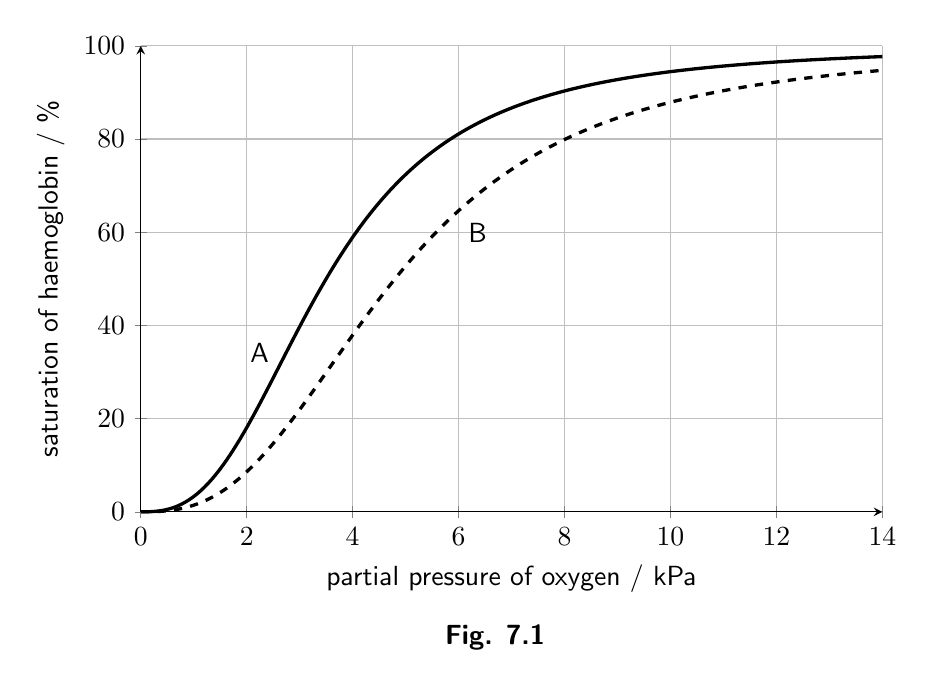
\begin{tikzpicture}[font=\sffamily]
  \begin{axis}[
    width=11cm, height=7.5cm, clip=false,
    axis lines=left, xmin=0, xmax=14, ymin=0, ymax=100,
    xtick={0,2,...,14}, ytick={0,20,...,100}, grid=major,
    xlabel={partial pressure of oxygen / kPa}, ylabel={saturation of haemoglobin / \%},
  ]
    \addplot[very thick, domain=0:14, samples=200] {100*x^2.7/(x^2.7+3.5^2.7)};
    \addplot[very thick, dashed, domain=0:14, samples=200] {100*x^2.7/(x^2.7+4.8^2.7)};
    \node[above left] at (axis cs:2.6,30) {A};
    \node[below right] at (axis cs:6,64) {B};
  \end{axis}
  \node[font=\sffamily\bfseries] at (4.5,-1.6) {Fig. 7.1};
\end{tikzpicture}
